\chapter{Results}
This section will present the results of the measurements with ZnTe and GaP as emitter crystals.
Calculations will be made to determine the electricfield strength of the produced $\si{\tera\hertz}$ radiation aswell as the Power of said radiation.
Futher a comparission between the different spectras of ZnTe and GaP will be shown and the efficiency in producing radiation will be discussed.

\section{Zinc telluride}
For this measurments a $\SI{1}{\milli\meter}$ thick ZnTe crystal is used as the emitter.
Another $\SI{1}{\milli\meter}$ thick ZnTe crystal is used as the detector.
The measurements are taken as described in section \ref{sec:execution}.
At this point it should be said, that the Znte crystal that is used as the emitter has two burn marks on it.
The burned crystal can be seen in figure \ref{fig:ZnTe_burned}.
Obviously the burned part of the crystal negatively effects the efficiency of $\si{\tera\hertz}$ production.
Which is why the part of the laser with the highest power is not focused on the burned part.
Still some of the laser hits the burned part of the crystal.
\\\\
To develop an understanding for the data the first figure that should be looked at is the time resolved EOS data.
For this the lock-in Amplifier output is plotted against the time delay between pump and probe beam.
The figure \ref{ZnTe:2_11_30_20_signal} shows the resulting plot.
This measurement is taken with a pump power of $\SI{135.0}{\milli\W}$, which is the highest pump power that is used.
The typical trend of a $\si{\tera\hertz}$ pulse can clearly be seen.
\\
Before the pulse starts the signal is balanced at $X(V)=0$.
\begin{figure}
    \centering
    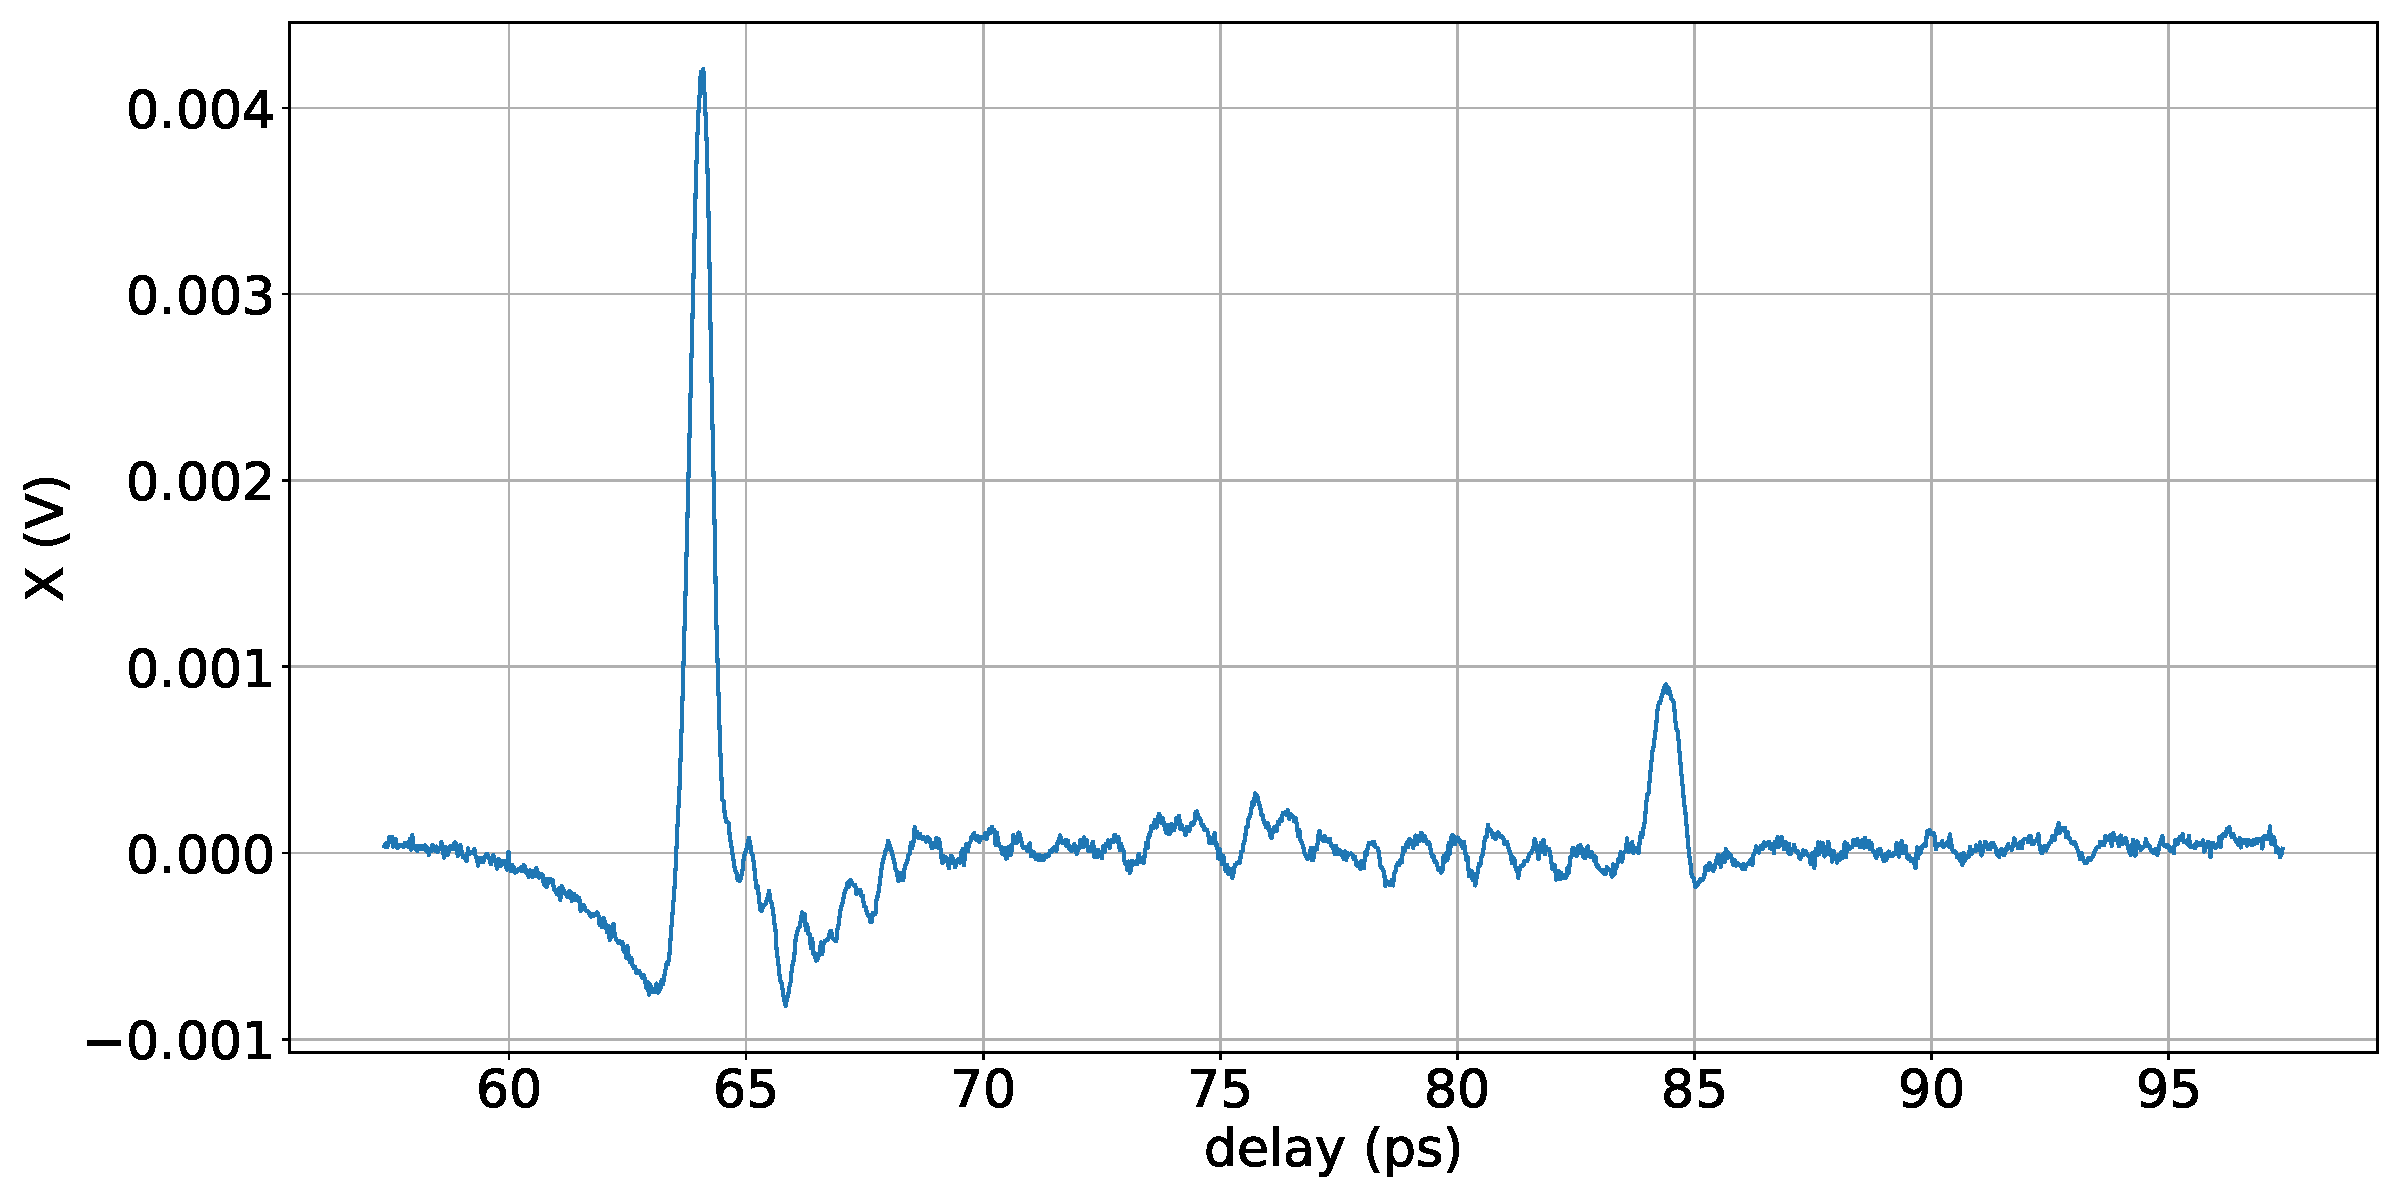
\includegraphics[width=0.75\textwidth]{Plots/2_11_30_20normalX.pdf}
    \caption{The $\si{\tera\hertz}$ pulse, that is measured by EOS, with a pump power of $\SI{135.0}{\milli\W}$.
    The EOS signal is plotted against the delay in $\si{\pico\second}$.
    A post pulse can be seen at a delay of $\SI{84}{\pico\second}$.}
    \label{ZnTe:2_11_30_20_signal}
\end{figure}
At a delay of about $\SI{58}{\pico\second}$ the pulse starts, which manifests in an increasingly negativ $X(V)$ value.
After about $\SI{5}{\pico\second}$ behind the start, the minimum is reached with an $X(V)$ value of $\SI{-0.746}{\milli\V}$ after which the lock-in Amplifier output increases drastically up to a value of $\SI{4.206}{\milli\V}$.
Here the maximum of the plot is reached, which corresponses to the maximum $\si{\tera\hertz}$ electricfield strength inside the detector crystal.
After the maximum the signal drops almost to zero.
\\
From this point on there are some oszillations, but no major features are visible. %are those oszialltions acuatlly caused by water?
Up until a delay of $\SI{84}{\pico\second}$, where the post pulse starts.
The post pulse is caused by reflections of the $\si{\tera\hertz}$ pulse inside the crystal.
Which is why the post pulse is just an echo of the intial pulse and thus alters the signal in a negativ way.
For futher calculations the data that is taken up until the post pulse will be used.
\\\\
\FloatBarrier
To confirm that the pulse that is shown in figure \ref{ZnTe:2_11_30_20_signal} actually corresponses to a $\si{\tera\hertz}$ pulse a Fourier-Transformation of the data is calculated. %Do I need to mention FFT in theory?
Because the Fourier-Transformation is done numerically the FFT function of the python package scipy \cite{scipy} is used.
The resulting Fourierspectrum is shown in figure \ref{fig:2_11_30_20_fft}.
The Spectrum is also plotted against a logarithmic y-axis, which results in the plot in figure \ref{fig:2_11_30_20_fft_log}.
\\
With this it is easy to confirm that the produced radiation actually lies in the $\si{\tera\hertz}$ regime.
Most of the radiation that is produced has a frequenzy between $0.3-1.1\,\si{\tera\hertz}$, but radiation with even higher $\si{\tera\hertz}$ frequencies is produced aswell.
Espacially in the spectrum which is plotted against the logarithmic y-axis the water absorption line of $\SI{1.226}{\tera\hertz}$ is clearly visible.
This is due to the water vapor in the air between emitter and detector crystal.
Some absorption lines at even higher frequencies are visible too.
\begin{figure}%
    \caption{The Fourierspectrum of the data from ZnTe, that is collected with the highest pump power of $\SI{135.0}{\milli\W}$.
    One of the spectras is plotted against a logarithmic axis to see the higher frequencies aswell.}%
    \begin{subfigure}{\columnwidth}%
        \centering
        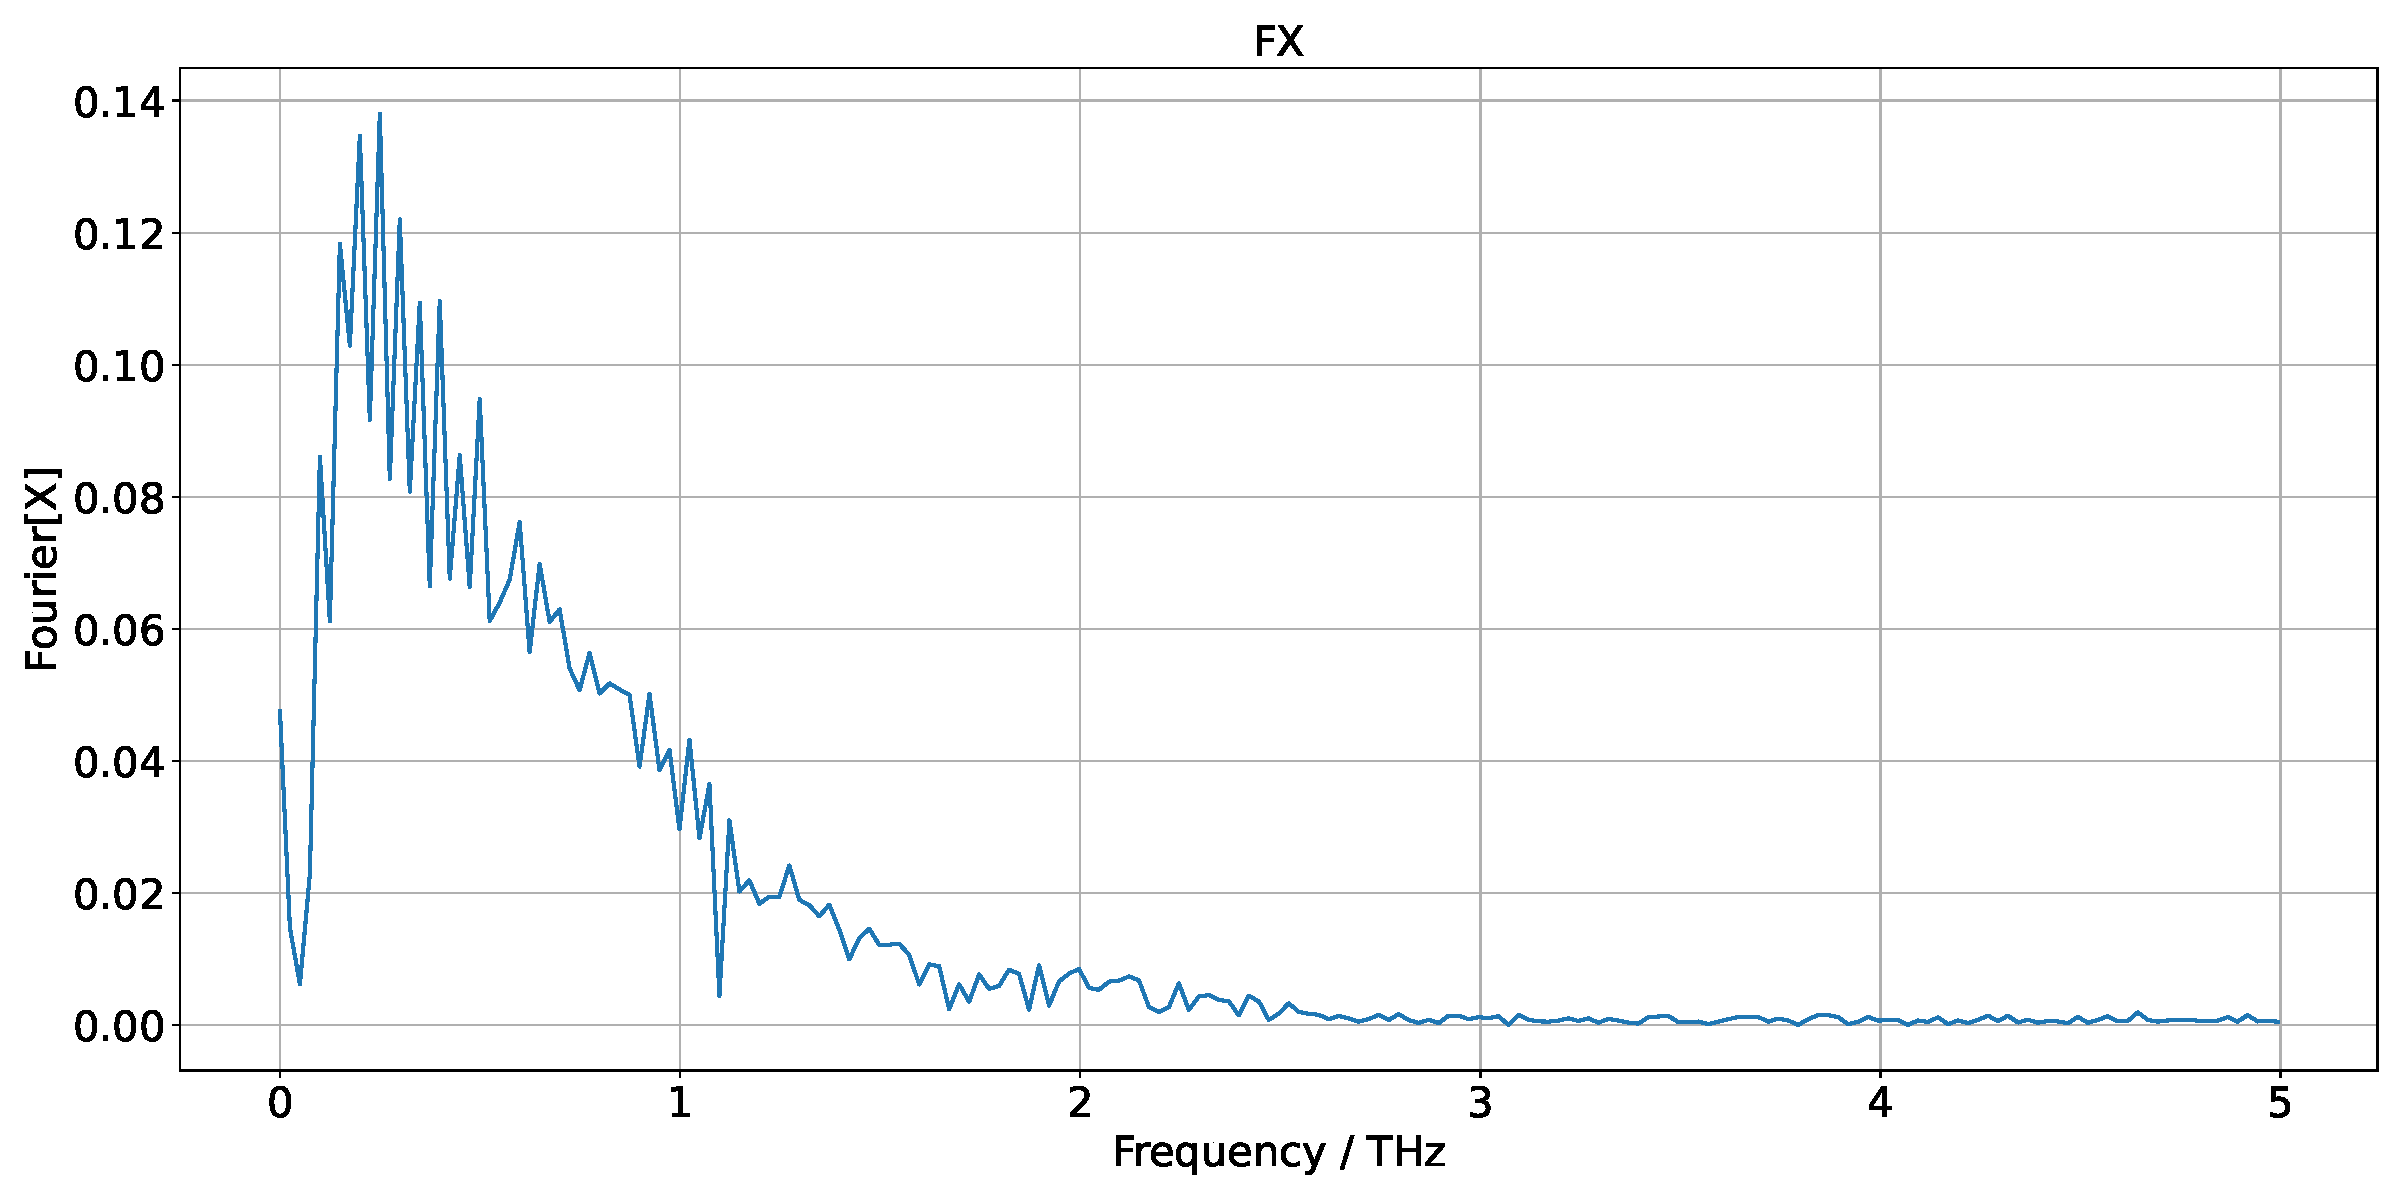
\includegraphics[height=3.5cm]{Plots/2_11_30_20normalFX.pdf}%
        \caption{The Fourier-Transformation of the $\si{\tera\hertz}$ pulse shown in figure \ref{ZnTe:2_11_30_20_signal}.
        It can clearly be seen that the frequency of the radiation lies in the lower $\si{\tera\hertz}$ regime.}%
        \label{fig:2_11_30_20_fft}%
        \end{subfigure}%
    \hfill% Fills available space in the center -> space between figures
        \begin{subfigure}{\columnwidth}%
        \centering
        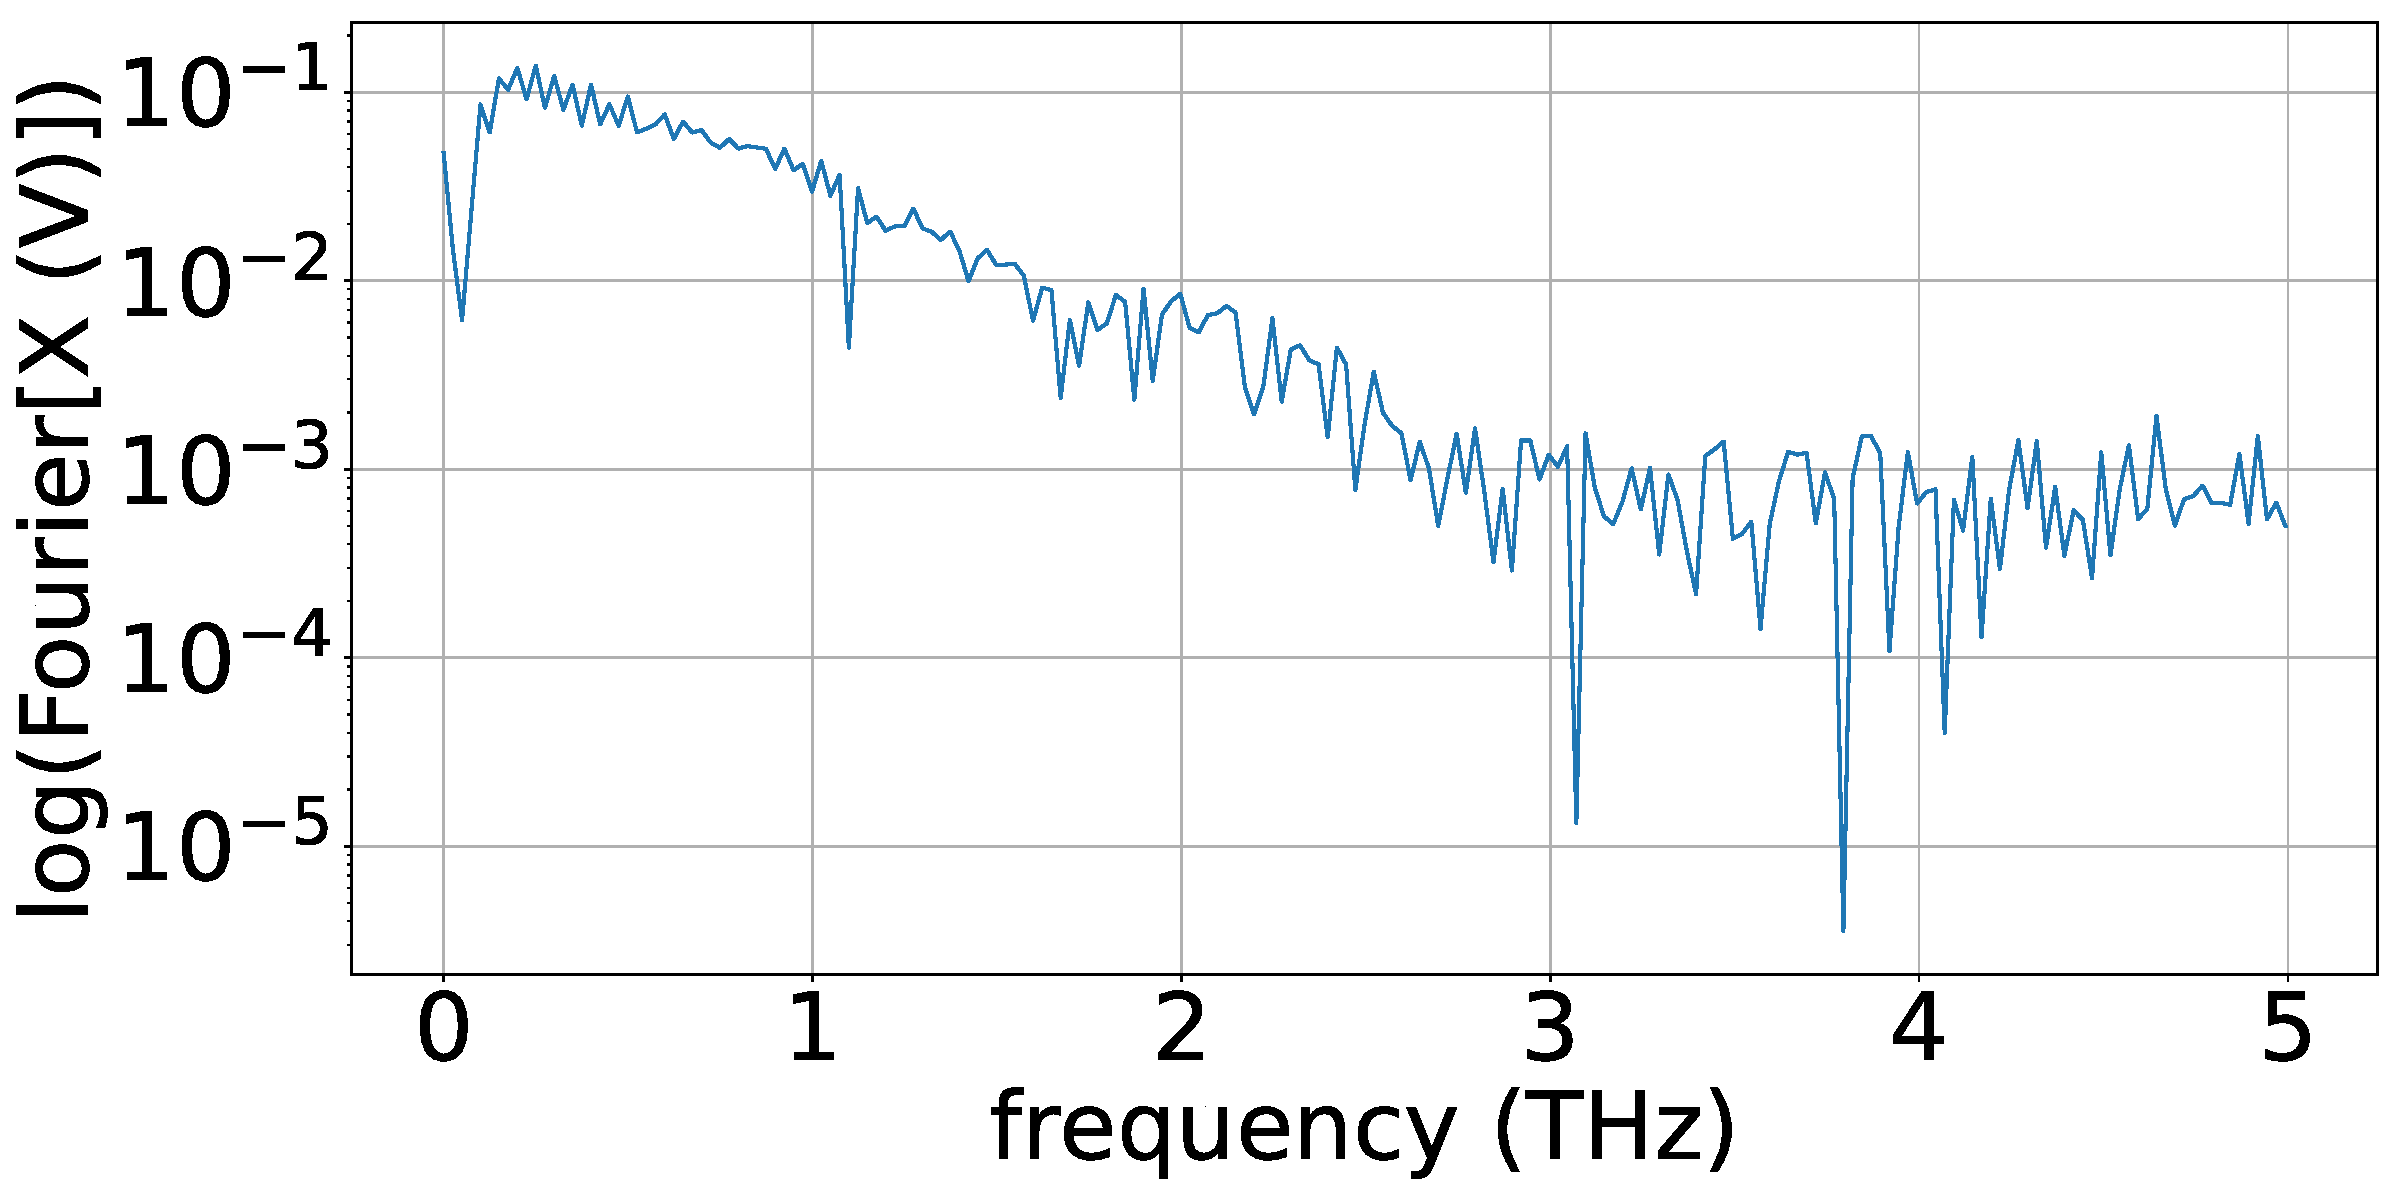
\includegraphics[height=3.5cm]{Plots/2_11_30_20normallog(FX).pdf}%
        \caption{The Fourierspectrum of the data shown in figure \ref{ZnTe:2_11_30_20_signal} plotted against a logarithmic y-axis.
        This shows that higher $\si{\tera\hertz}$ frequencies are produced aswell. Some absorption lines can also bee seen.}%
        \label{fig:2_11_30_20_fft_log}%
    \end{subfigure}%
    \label{fig:fourier_znte}%
\end{figure}%
\FloatBarrier
\subsection{Electric field measurments}
\label{sec:znte_electricfield}
\FloatBarrier
To determine the peak electricfield of the $\si{\tera\hertz}$ pulse, several measurements of $A$, $B$ and $A-B$ are taken as described in section \ref{sec:field}.
To get the best result and minimize the error through noise for $A$ and $B$, their value is measured $500$ times.
After the data is taken their mean value is used for futher calculations with their error being the standard deviation.
\\
All futher errors are calculated with the python package uncertainties \cite{uncertainties}, which uses the standard gaussian error propagation theory described in section \ref{sec:error}.
With those the electricfield, for every $A-B$ value that is measured, is calculated by equation \ref{eq:electricfield_A_B}.
All the peak electricfield values are than collected and plotted against their corresponding pump power.
The resulting plot can be seen in figure \ref{fig:znte_electricfield}.
\\
\begin{figure}
    \centering
    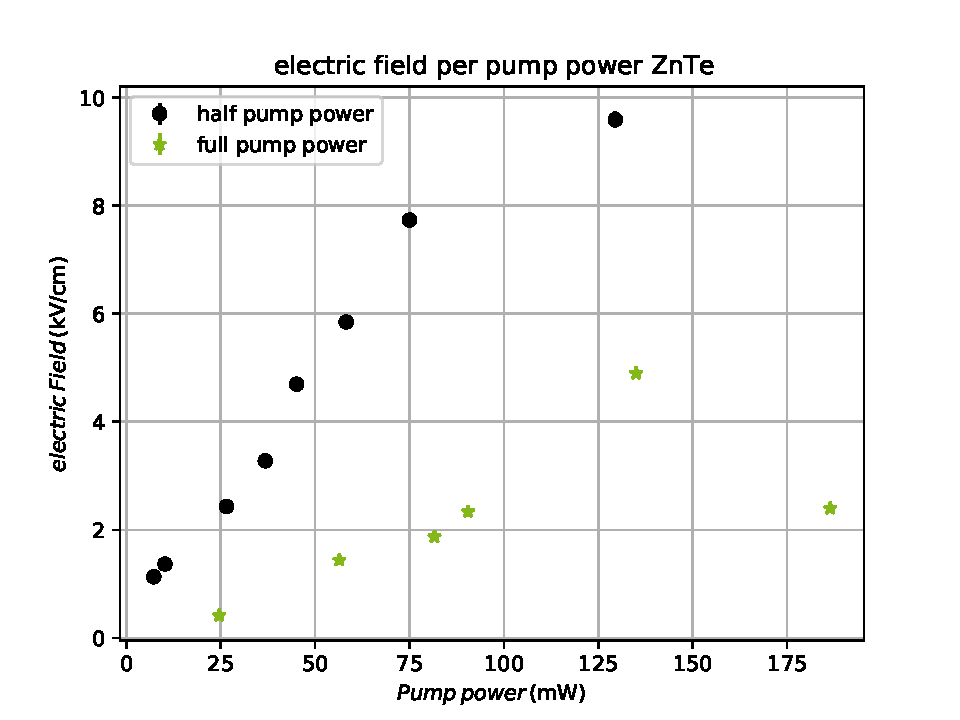
\includegraphics[width=0.5\textwidth]{Plots/eltric_field_ZnTe.pdf}
    \caption{The calculated peak electricfield of the $\si{\tera\hertz}$ pulse is plotted against its corresponding pump laser power.
    Diffrent initial laser powers are shown through diffrent colors. The high power being $\SI{579}{\milli\W}$ the lower being $\SI{291}{\milli\W}$.
    A linear regression of the calculated values is plotted in blue.}
    \label{fig:znte_electricfield}
\end{figure}
Because the laser power that the setup receives right at the beginning changes from $\SI{579}{\milli\W}$ to $\SI{291}{\milli\W}$, over the course of the measurement, the values that are taken with the higher initial laser power are marked with green stars.
The lower initial laser power of $\SI{291}{\milli\W}$ is marked with black dots.
A linear regression is done with the formula
\begin{equation}
    f(x) = mx + b,
    \label{eq:linear}
\end{equation}
where $x$ are the pump power values and $f(x)$ are all the peak electricfield values.
The calculation are done with the function \textbf{curve\_fit} from the python package scipy \cite{scipy}.
It returns the fit parameters 
\begin{align*}
    m =& 0.0189\\
    b =& 0.2615
    vielleicht sollte ich kein align nutzen auch wenn es am besten aussieht. das nimmt einfach zu viel platz weg
\end{align*}
with which the linear fit is plotted.
Espacially for lower pump powers the peak electricfield values follow the linear trend.
However at higher pump powers the calculated electricfield values diverge heavily from the linear fit.
\\
A probable cause is that at higher pump powers the burned part of the crystal influeces the production of $\si{\tera\hertz}$ much stronger.
The linear trend is in good comparission with the literature \cite{electric_field_compare}, which also shows a linear trend at lower pump power/pulse energys.
However the electricfield strength is way lower than in the literature.
The maximum electricfield strength that is calculated is $\SI{4.900(19)}{\kilo\V\per\centi\meter}$, which corresponses to a pump power of $\SI{135.0}{\milli\W}$.
\\
This is not actually the highest pump power that is used.
The expectation would be that the highest pump power corresponses to the highest peak electricfield.
The reason for this annomaly, aswell as the lower electricfield strength compared to the literature, might be the smaller thickness of the crystal as well as the lower quality of the crystal due to its burned spots.
\FloatBarrier
\subsection{Power measurments}
\FloatBarrier
To calculate the peak electricfield power of the $\si{\tera\hertz}$ pulse the spotsize of the pulse is measured.
The spot has a radius of $\SI{2.5}{\milli\meter}$ according the aperature opening.
If a circular spot is assumed the spot area is $\SI{19.62}{\milli\meter\squared}$.
With the electricfield values that are calculated in section \ref{sec:znte_electricfield} the intensity can then be calculated according to equation \ref{eq:intensity}.
Now all variables to calculate the $\si{\tera\hertz}$ electricfield power are known and just need to be plugged into equation \ref{eq:power}.
\\
The resulting power values are then plotted against their corresponding pump powers and shown in figure \ref{fig:znte_power}.
\begin{figure}
    \centering
    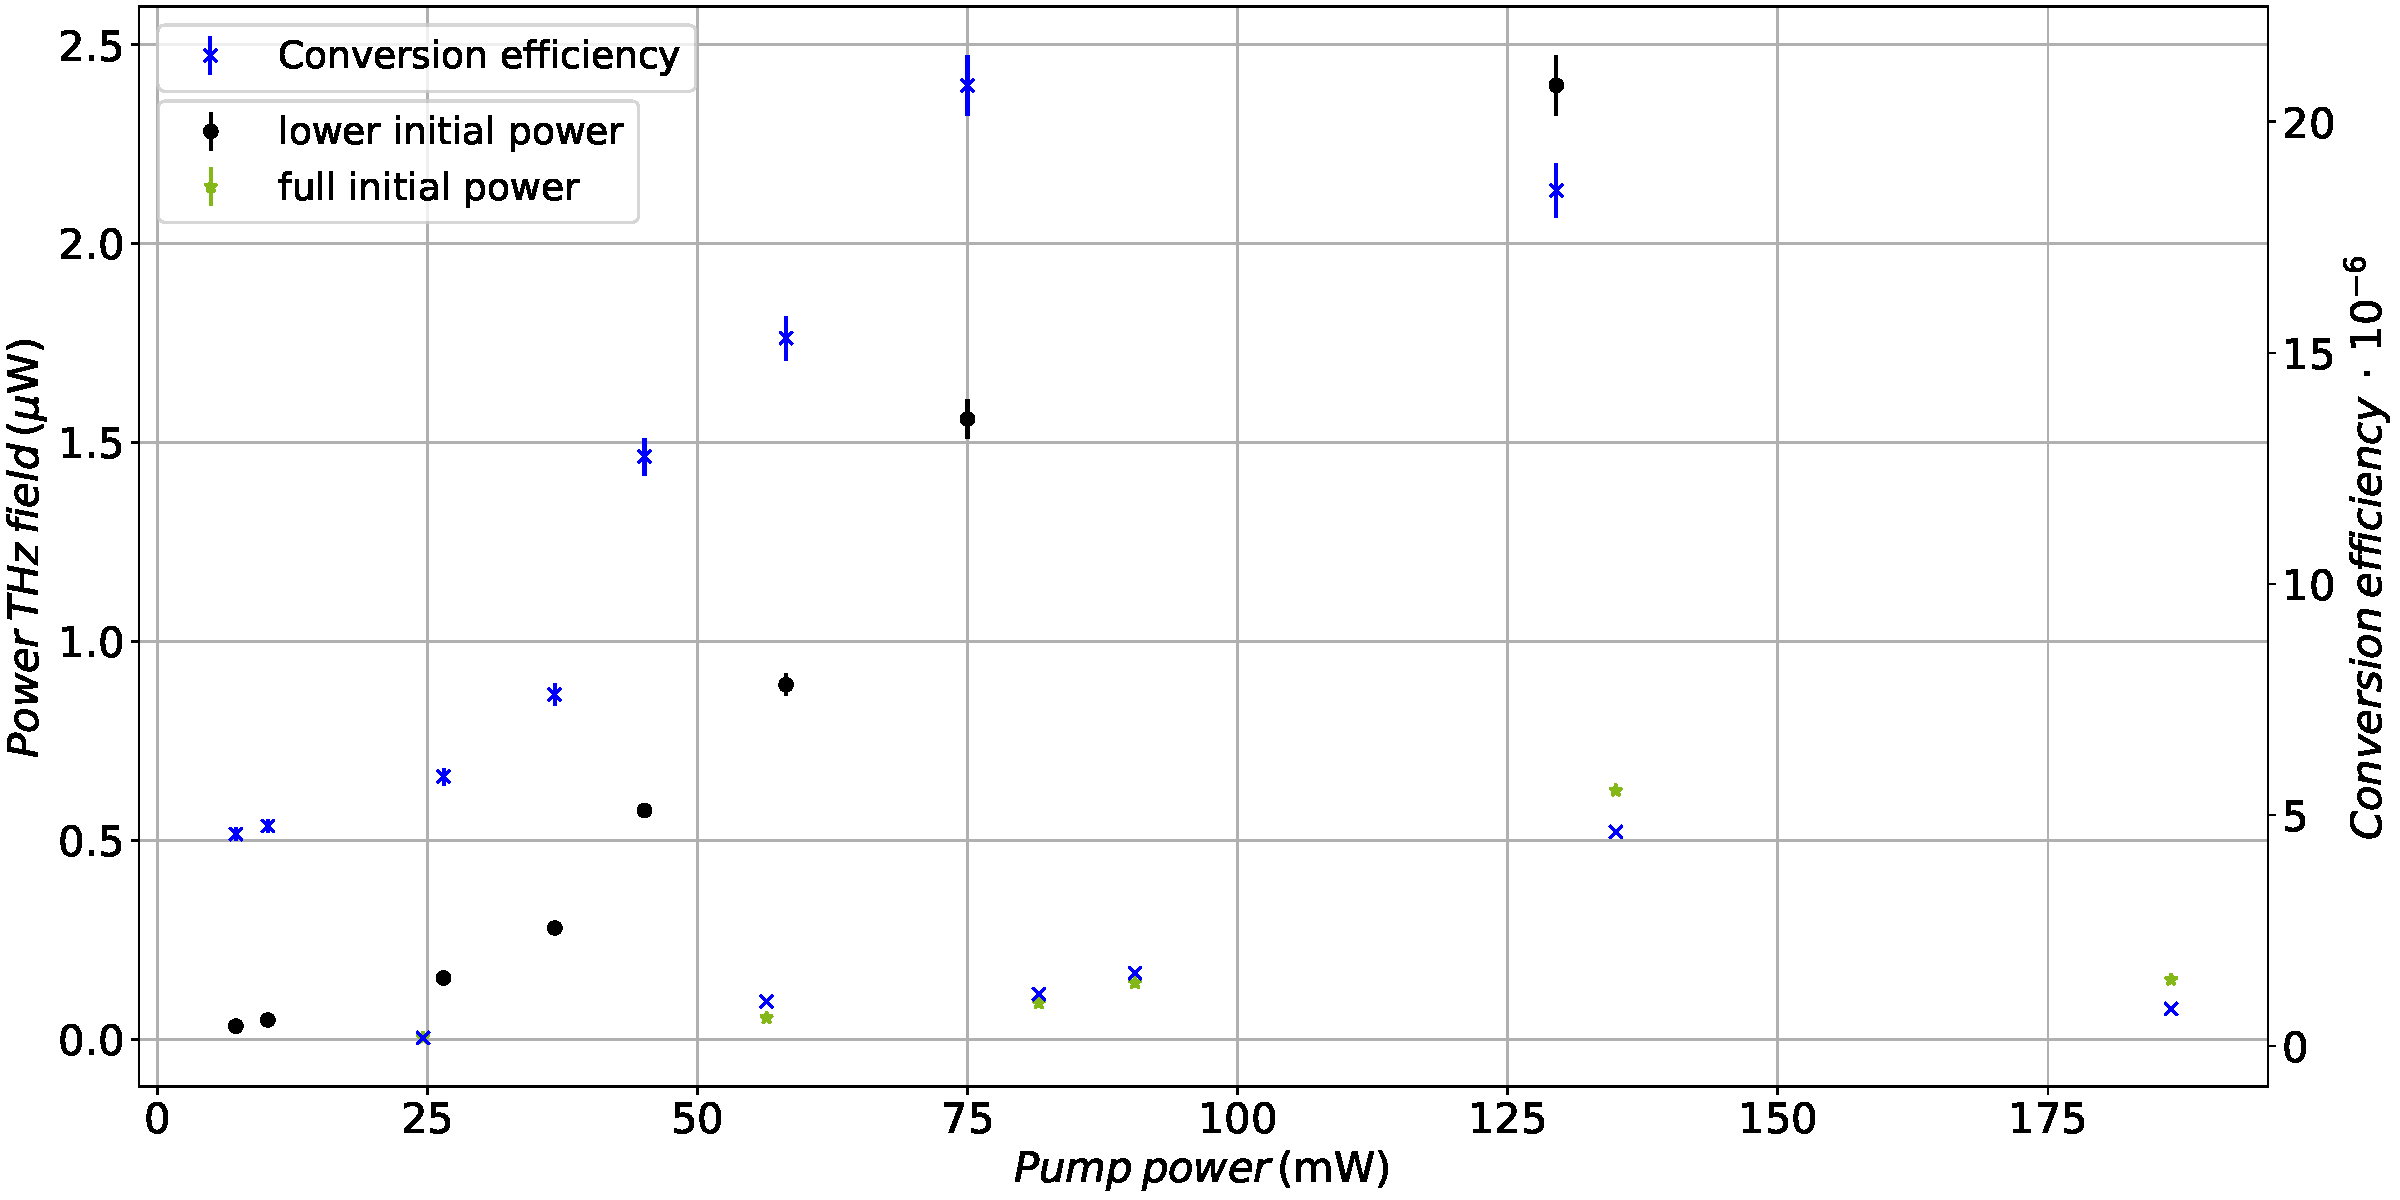
\includegraphics[width=\textwidth]{Plots/Powerznte.pdf}
    \caption{The calculated peak electricfield powers of the $\si{\tera\hertz}$ pulses are plotted against their corresponding pump powers.
    Because the initial laser powers that are fed into the setup change over the course of the measurement, the different laser power are marked with green stars, for the higher power, or black dots, for the lower power.
    The high initial laser power has a value of $\SI{579}{\milli\W}$, the lower a value of $\SI{291}{\milli\W}$.
    A conversion efficiency from pump power to $\si{\tera\hertz}$ power is calculated and shown as blue crosses.}
    \label{fig:znte_power}
\end{figure}
Because the initial laser power that comes into the setup changes the different laser powers are marked with green starts, for high power, and black dots, for lower power.
The high initial power has a value of $\SI{579}{\milli\W}$, the lower a value of $\SI{291}{\milli\W}$.
\\
A conversion efficiency from laser pump power to $\si{\tera\hertz}$ peak electricfield power is calculated and plotted as blue crosses in figure \ref{fig:znte_power}.
It is calculated by 
The calculated peak electricfield power of the $\si{\tera\hertz}$ pulse, shows a linear trend up until a pump power of $\SI{90.5}{\milli\W}$.
Here the peak electricfield power has a value of $\SI{0.1421(11)}{\micro\W}$.
\\
With pump powers that are even greater than $\SI{90.5}{\milli\W}$ the peak electricfield power of the $\si{\tera\hertz}$ pulse does not increase.
The only exception for that is at a pump power of $\SI{135.0}{\milli\W}$ with a peak electricfield power of $\SI{0.6255(46)}{\micro\W}$.
This exception is most probably an error in the measurement and does not really reflect the behavior of the emitter crystal.
%or maybe this would be the real behavior if the crystal is not burned. so that the power would rise linearly for even longer.
\\\\
The conversion efficiency lies between $\SI{2.544(19)e-07}{}$ for a pump power of $\SI{7.28}{\milli\W}$ and $\SI{4.634(35)e-06}{}$ with a pump power of $\SI{135.0}{\milli\W}$
It shows a linear increasing trend with rising pump power.
The trend stops at a pump power of $\SI{90.5}{\milli\W}$ after which the conversion efficiency stays constannt except for one value.
Just like the peak electricfield power, this value corresponses to a pump power of $\SI{135.0}{\milli\W}$.
The conversion efficiency for this pump power is $\SI{4.634(35)e-06}{}$.
\\\\
A comparisson with the literature is quite hard, because most other setups use pump powers that are higher than the once reached in this setup.
However the measurements from the paper \cite[5]{THZ_eltric_field} shows a similar trend at low pulse energys per area.
Pump power can easily be converted into pulse energy per area, just by multiplying with the pump laser spot size on the emitter crystal and divinding by the number of pulses per second.
The pulse energy per area can be seen in the additional x-axis in figure \ref{fig:znte_power}.
\\
\textbf{doppelte x achse für plot, ich weiß nur noch nicht ob das ganz richtig ist.}  
This shows that the conversion efficiency of this setup is about ten times lower than in the said paper.
The most probable reason for that are the burned parts of the crystal, that lowers the efficiency of the crystal.
The conversion from pump power to pulse energy per unit area is also just a rough estimation because the laser power is not equally distrubuted over the laser spot, but rather follows a gaussian distrubution.
It is to be expected that a lot of the laser power also does not even hit the crystal because the lens, that is positioned infront of the crystal, focuses the beam not enough for all the beam power to hit the crystal.
This results in some laser power hitting the holder of the ZnTe crystal.
The reason for not focusing down enough is to avoid reaching the damage threshold of the crystal as it is already damaged.
\FloatBarrier
\section{Gallium phosphide}
As emitter crystal a $\SI{0.3}{\milli\meter}$ GaP crystal is used.
A $\SI{1}{\milli\meter}$ ZnTe crystal is in use as the detector crystal.
The measurements and prepartions are the same as for ZnTe and a detailed description can be found in section \ref{sec:execution}.
A first look at the data that is collected can be taken in figure \ref{fig:GaP14_55_42normalX}.
\\
\begin{figure}
    \centering
    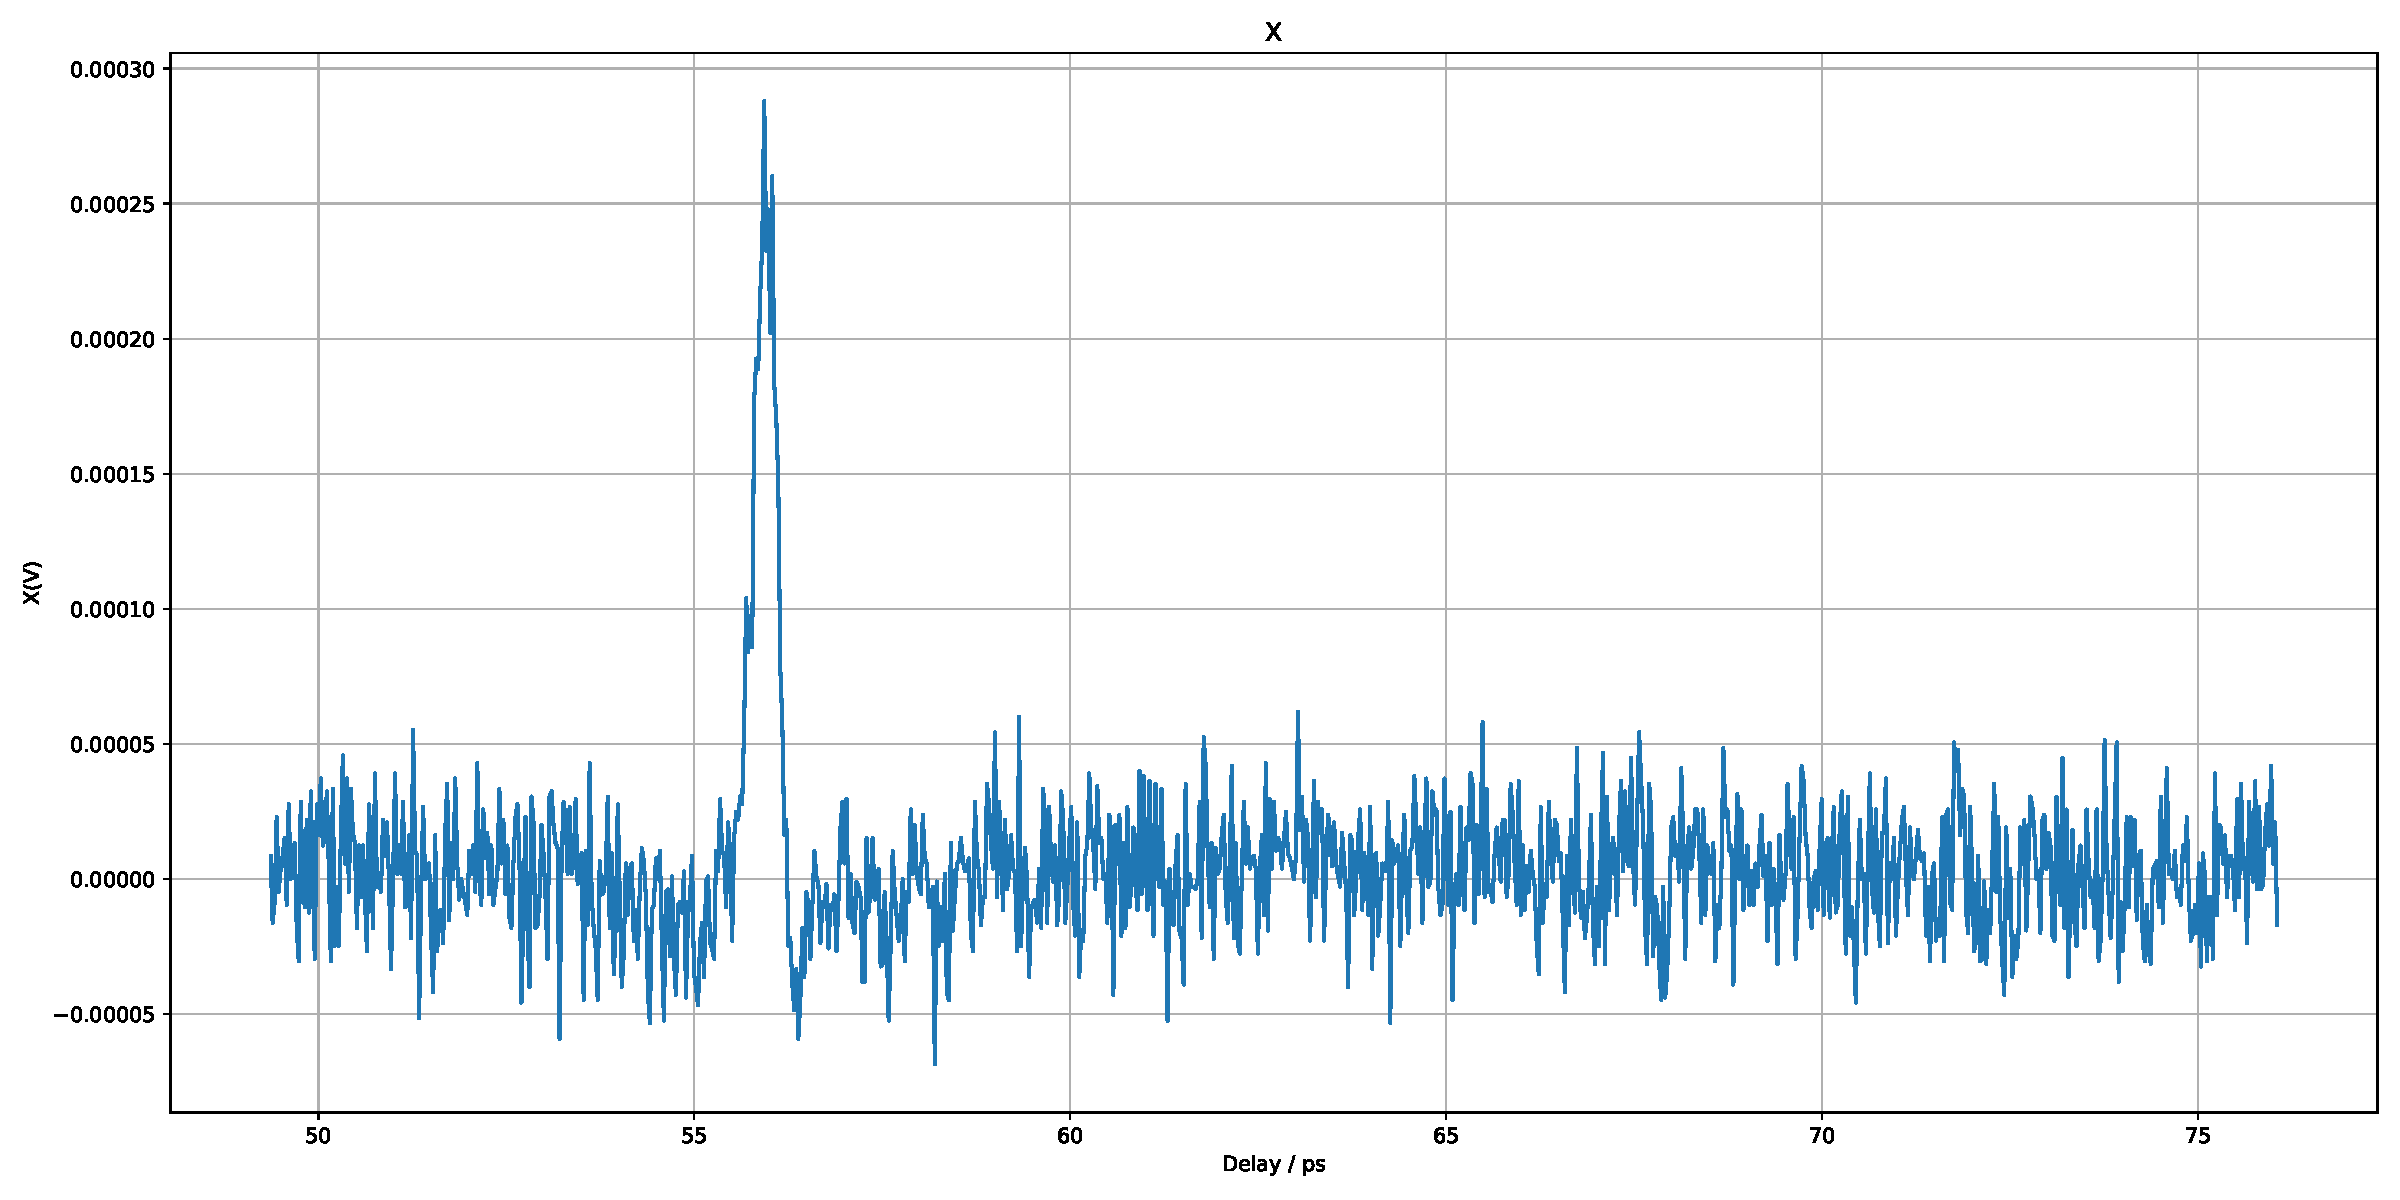
\includegraphics[width=0.75\textwidth]{Plots/GaP14_55_42normalX.pdf}
    \caption{The EOS data that is collected with GaP as emitter crystal with an applied laser pump power of $\SI{124.2}{\milli\W}$, which is the highest laser pump power that is measured.}
    \label{fig:GaP14_55_42normalX}
\end{figure}
At the start of the measurement the signal is distrubuted around zero, but not totally zero because of the noise.
Around $\SI{54}{\pico\second}$ a downward trend can be seen, which reaches its minimum at $\SI{55}{\pico\second}$.
Then the signal gradient becomes positive and increases in a very short interval up to a peak value of $\SI{0.287}{\milli\V}$ at a delay of $\SI{55.9}{\pico\second}$.
\\
After the peak the signal drops down again into another minimum with a value of $\SI{-59.128}{\micro\V}$ at a delay of $\SI{56.3}{\pico\second}$.
Now the signal raises back to zero and shows no further significant features until the end of the measurement.
This measurement does not show any post pulse feature.
\\\\
A Fourier-Transformation is calculated, which is shown in figure \ref{fig:GaP14_55_42_fft}.
The Fourierspectrum has also been plotted against a logarithmic y-axis to make absorption lines more visible and acquier more informations about the higher frequencies, that dont appear in the normal Fourierspectrum.
\\
This Fourierspectrum that is plotted against the logarithmic y-axis is shown in figure \ref{fig:GaP14_55_42_fft_log}.
There are no features in the Fourierspectrum that can be clearly recognized as absorption lines.
The Fourierspectrum shows a linear downward trend from its highest amplitude at a frequency of $\SI{0.3}{\tera\hertz}$ down to a frequency of $\SI{2.5}{\tera\hertz}$.
After $\SI{2.5}{\tera\hertz}$ the Spectrum stays almost constant in amplitude, which shows that the majority of the produced radiation lies between $0.3$ and $\SI{2.5}{\tera\hertz}$.

\begin{figure}%
    \caption{The Fourierspectrum of the data for GaP, that is collected with the highest pump power of $\SI{124.2}{\milli\W}$.
    One of the spectras is plotted against a logarithmic axis to better see absorption lines or other features aswell.}%
    \begin{subfigure}{\columnwidth}%
        \centering
        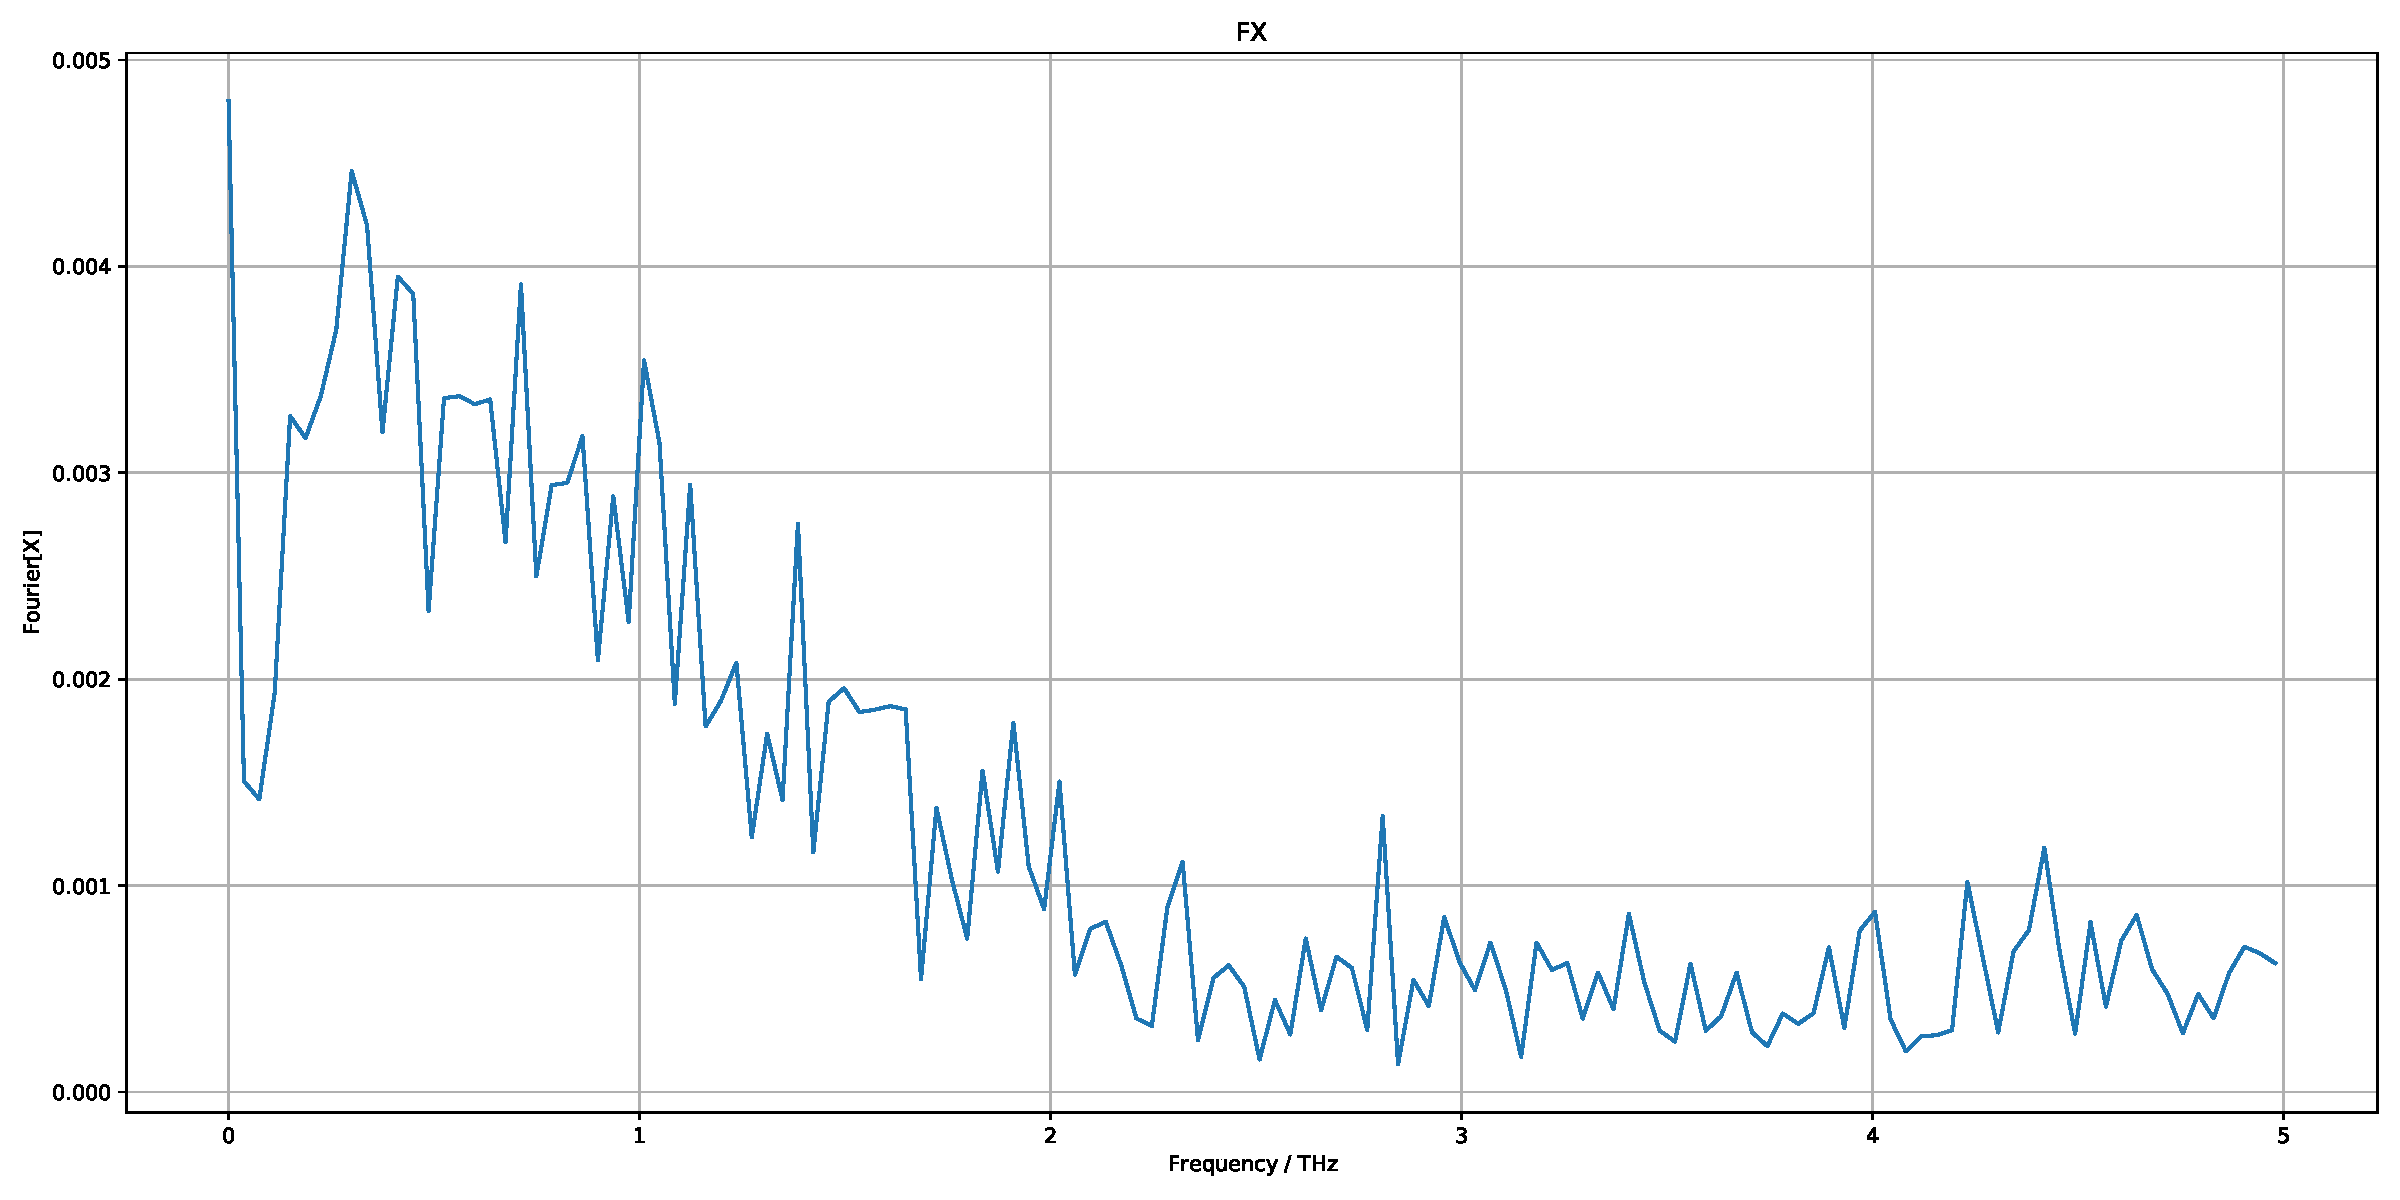
\includegraphics[height=3.5cm]{Plots/GaP14_55_42normalFX.pdf}%
        \caption{The Fourier-Transformation of the $\si{\tera\hertz}$ pulse shown in figure \ref{fig:GaP14_55_42normalX}.
        The Fourierspectrum shows a linear downward trend from $\SI{0.3}{\tera\hertz}$ to $\SI{2.5}{\tera\hertz}$.
        After which the spectrum stays almost constant at an value of $0.0005$.}%
        \label{fig:GaP14_55_42_fft}%
        \end{subfigure}%
    \hfill% Fills available space in the center -> space between figures
        \begin{subfigure}{\columnwidth}%
        \centering
        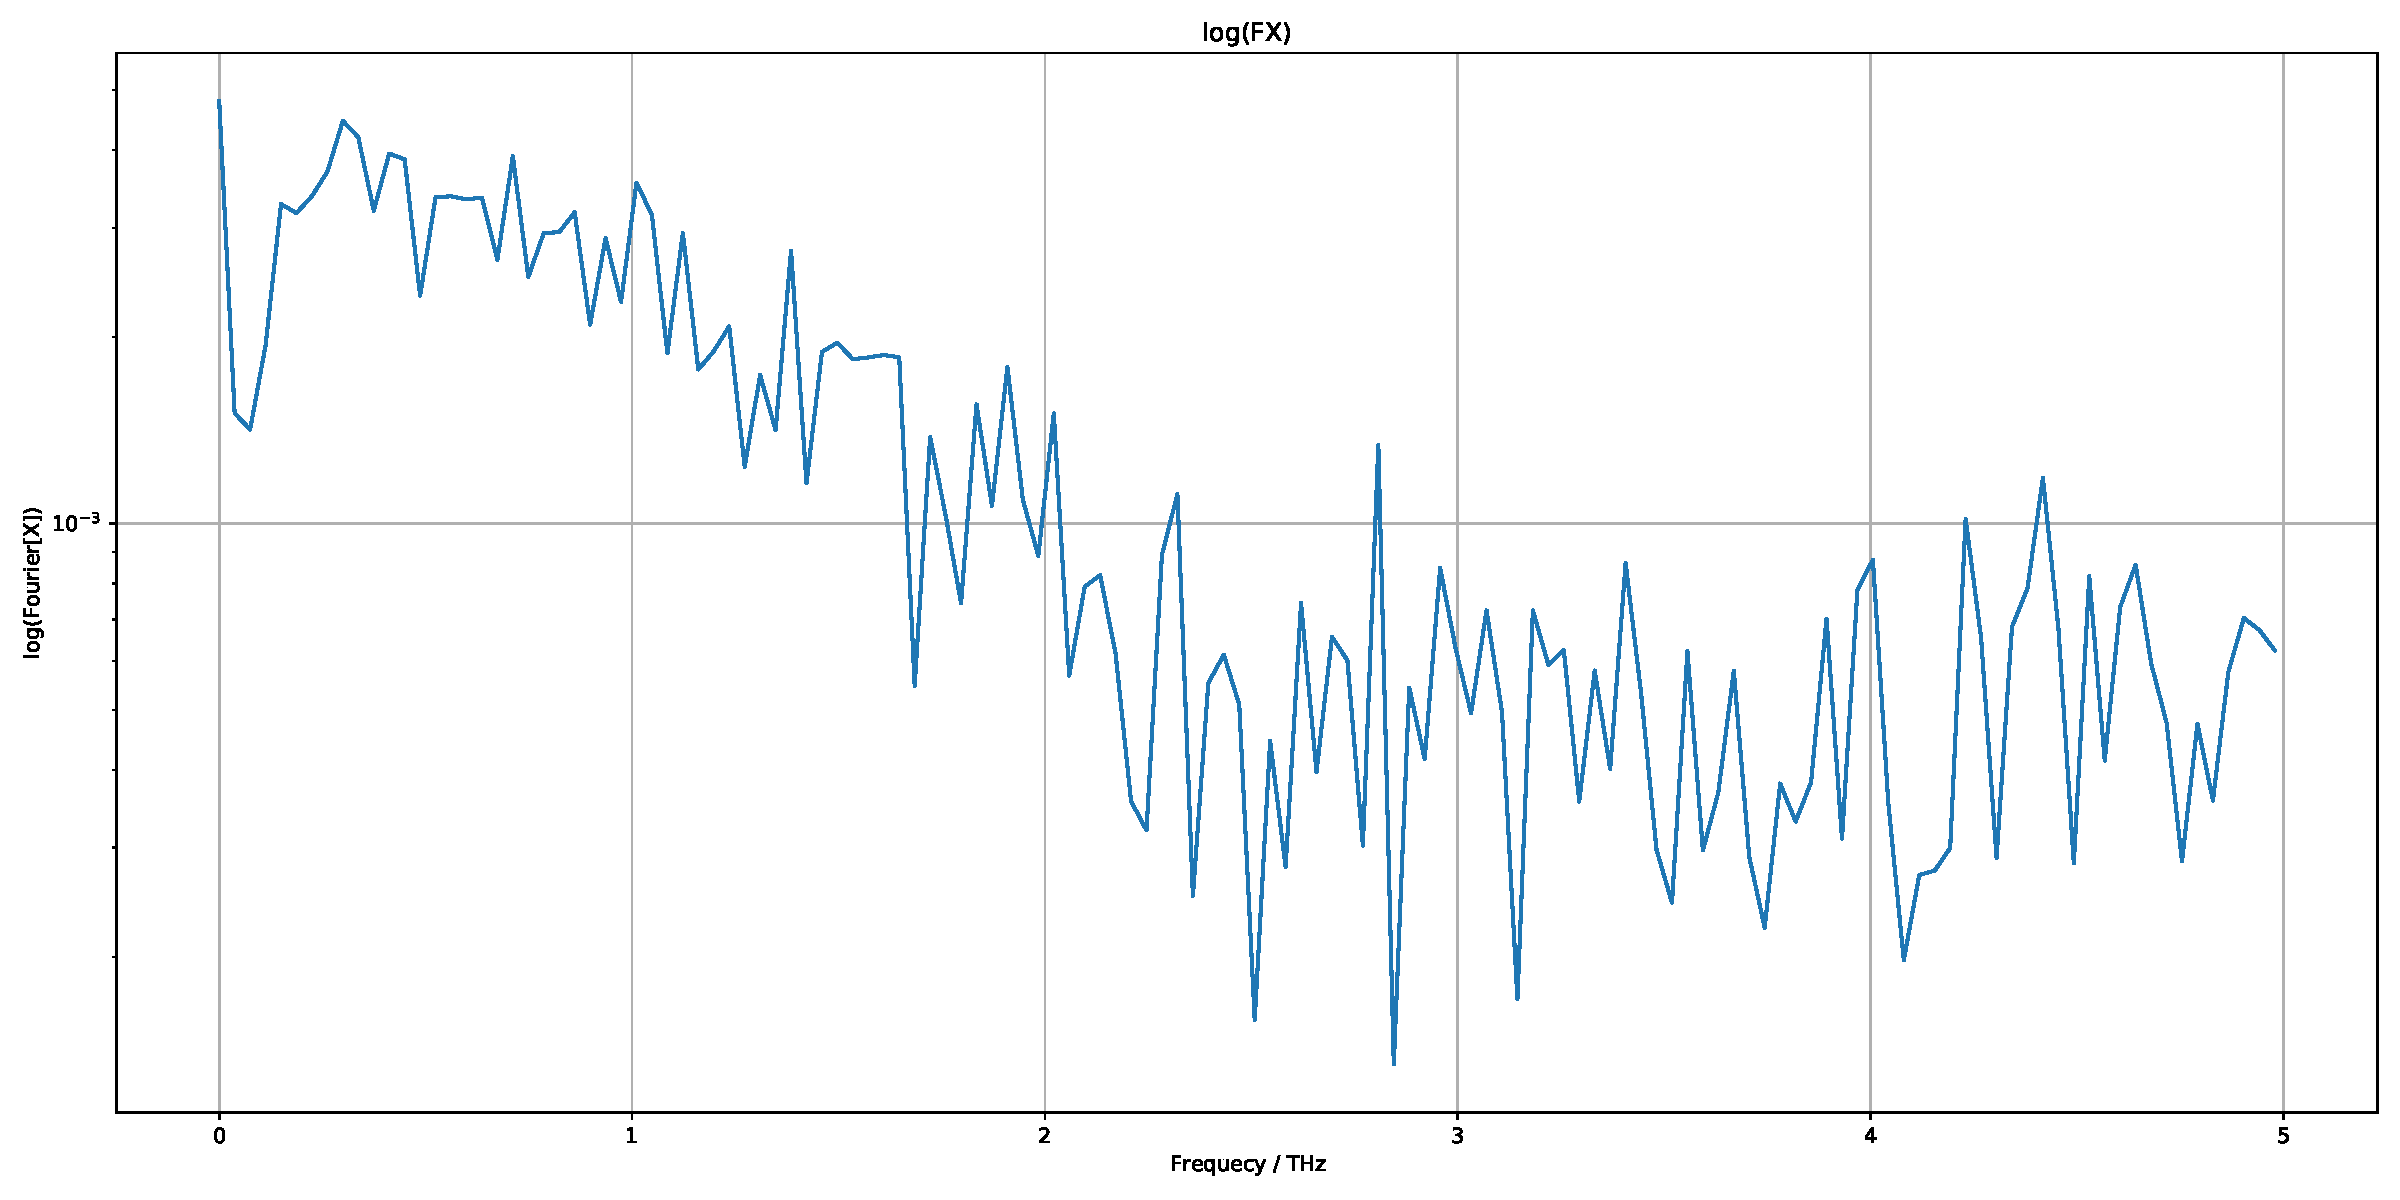
\includegraphics[height=3.5cm]{Plots/GaP14_55_42normallog(FX).pdf}%
        \caption{The Fourierspectrum of the data shown in figure \ref{fig:GaP14_55_42normalX} plotted against a logarithmic y-axis.
        There are no absorption lines recognizable in the plot.}%
        \label{fig:GaP14_55_42_fft_log}%
    \end{subfigure}%
    \label{fig:fourier_znte}%
\end{figure}%
\FloatBarrier
\subsection{Electric field measurments}
\FloatBarrier
The electricfield is measured as described in section \ref{sec:field}.
As emitter crystal a $\SI{0.3}{\milli\meter}$ GaP crystal is used.
The detector is an $\SI{1}{\milli\meter}$ ZnTe crystal.
To lower the error through noise the values $A$ and $B$ are measured $500$ times.
The median of each dataset is used for further calculation.
The error is given by the standard deviation of the median.
\\
To calculated the peak electricfield the positive peak $A-B$ values, which are taken by each measurement are plugged into equation \ref{eq:electricfield_A_B}.
The peak electricfields for every pump power are than plotted against there corresponding pump powers.
The resulting plot is shown in figure \ref{fig:gap_electricfield}.
\begin{figure}
    \centering
    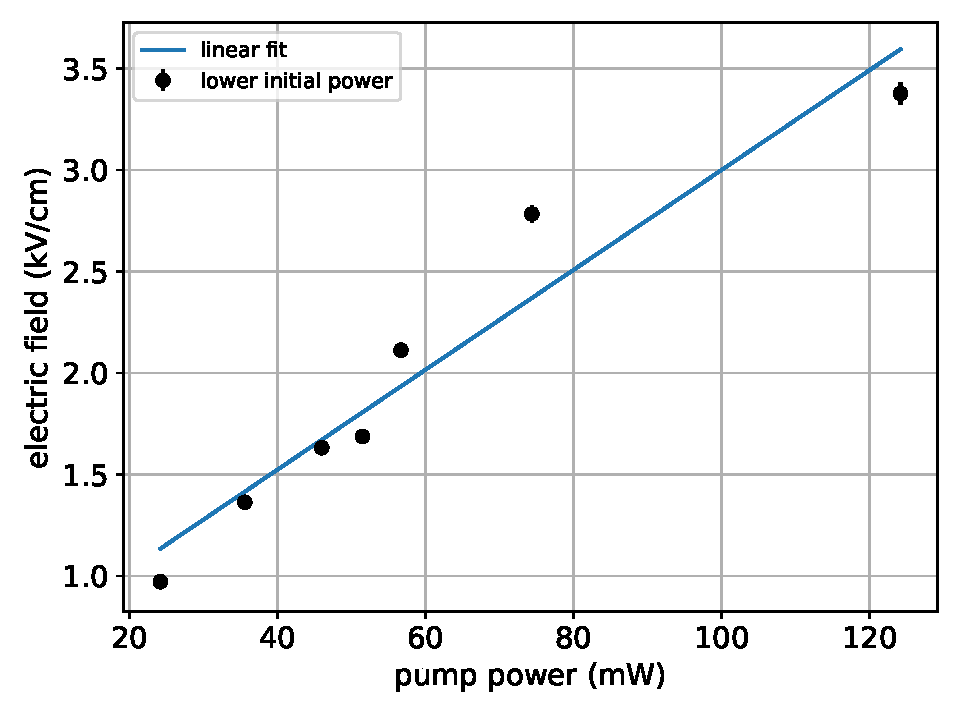
\includegraphics[width=0.5\textwidth]{Plots/eltric_field_GaP.pdf}
    \caption{The peak electricfield, marked as black dots, is plotted against its corresponding pump power.
    A linear fit, as filled blue line, for the plotted datapoints is also shown in the figure.}
    \label{fig:gap_electricfield}
\end{figure}
The calculated peak electricfields show a linear trend.
For this reason a linear regression is calculated for equation \ref{eq:linear}.
The regression is done with the function \textbf{curve\_fit} from the python package scipy.
Said function returns the parameters
\begin{align*} 
    m =& 0.0245\\
    b =& 0.5403
\end{align*}
which are used to make the linear fit shown in figure \ref{fig:gap_electricfield}.
\textbf{hier brauch ich noch literatur für GaP THz electric field}.
\\
The linear regression shows that the datapoints actually follow a linear trend.
At higher pump powers the datapoints are more distancent from the linear fit.
The highest eletricfield of $\SI{3.38(5)}{\kilo\V\per\centi\meter}$ calculated, corresponses to a pump power of $\SI{124.2}{\milli\W}$, which is the highest laser pump power that is used.
This follows the linear trend \textbf{and is in good comparission with the literature?}.

\textbf{It is also intersting that even with very low pump powers $\si{\tera\hertz}$ radiation can still be produced.
In this case a pump power of $\SI{24.2}{\milli\W}$ is sufficient to produce a peak electricfield of $\SI{0.97(1)}{\kilo\V\per\centi\meter}$.}
\FloatBarrier
\subsection{Power measurments}

\FloatBarrier
\section{Comparisson}
Because the GaP crystal is $\SI{0.7}{\milli\meter}$ thinner than the ZnTe crystal all comparissions that are done in this chapter only apply for this specific setup and may not apply universally.


GaP no post pulse
%I should put another GaP plot in the abstracted to show how noisy it is